\documentclass[a4paper,12pt]{article}
\usepackage[english,ukrainian,russian]{babel}
\linespread{1}
\usepackage{ucs}
\usepackage[utf8]{inputenc}
\usepackage[T2A]{fontenc}
\usepackage[paper=portrait,pagesize]{typearea}
\usepackage{amsmath}
\usepackage{bigints}
\usepackage{amsfonts}
\usepackage{graphicx}
\usepackage{amssymb}
\usepackage{cancel}
\usepackage{gensymb}
\usepackage{multirow}
\usepackage{rotate} 
\usepackage{pdflscape}
\usepackage{bigstrut}
\usepackage[pageanchor]{hyperref}
\usepackage{chngpage}
\usepackage{fancybox,fancyhdr}
\newcommand\tab[1][1cm]{\hspace*{#1}}
\newcommand{\RomanNumeralCaps}[1]{\MakeUppercase{\romannumeral #1}}
\usepackage[left=20mm, top=20mm, right=15mm, bottom=15mm, nofoot]{geometry}


\begin{document}
    \pagestyle{fancy}
    \fancyhead{}
    \fancyhead[R]{ФІ-12 Завалій Олександр}
    \fancyhead[L]{09.02.2023}
    \begin{center}
        \large{\textbf{Міністерство освіти і науки України\\
                Національний технічний університет України\\
                «Київський політехнічний інститут імені Ігоря Сікорського»\\
                Навчально-науковий Фізико-технічний інститут}}\\
        \hfill \break \hfill \break \hfill\break \hfill \break \hfill \break \hfill \break \hfill \break
        \hfill \break \hfill \break \hfill \break
        \begin{center}
            \normalsize{\textbf{ОПЕРАЦІЙНІ СИСТЕМИ\\
            Комп’ютерний практикум\\
            Робота №1}}
        \end{center}
    \end{center}
    \hfill \break \hfill \break \hfill \break \hfill \break \hfill \break \hfill \break \hfill \break
    \hfill \break \hfill \break \hfill \break \hfill \break 
    \begin{flushright}
        \large{ \hspace{35pt} Виконав:\\
            студент групи ФI-12\\
            Завалій Олександр\\} 
        \large{ \hspace{35pt} Перевірив:\\
        Кірієнко О.В.} 
    \end{flushright}
    \hfill \break \hfill \break \hfill \break \hfill \break \hfill \break \hfill \break \hfill \break
    \hfill \break
    \begin{center} \textbf{Київ-2023} \end{center}
    \thispagestyle{empty}

\newpage
    \begin{center}
        \section*{\bfseries{Робота №1.\\
        Структура файлової системи Linux,
        основні команди, команди роботи з файлами
    }}
    \end{center}
    \textbf{Мета:} \\
    \hangindent=1.5cm 
    \hangafter=+1 \noindent
    Оволодіння практичними навичками роботи в системі
    Linux. Знайомство із структурою файлової системи,
    основними командами роботи з файлами. \\
    \begin{center}
        \Large{Варіант №5}
    \end{center}
    Зміст індивідуального завдання:
    \begin{enumerate}
        \item Завантажтеся в систему під вашим користувацьким ім'ям.
        \item Поміняйте ваш пароль. Ваш новий пароль повинен включати в себе як 
        частину номер Вашої залікової книжки.
        \item Виведіть системну дату.
        \item Підрахуйте кількість рядків у файлі: \textbf{/etc/rsyslog.conf}.
        \item Виведіть на екран вміст відповідного файлу.
        \item Виведіть календар на \textbf{2000} рік.
        \item Виведіть календар на 1752 рік. Чи не помічаєте що-небудь цікаве у вересні? Поясніть.
        \item Визначте, хто ще завантажений у систему.
        \item Наберіть команду \textbf{ping}. Поясніть результат.
        \item Скопіюйте файли: \textbf{/bin/more}, \textbf{/bin/gzip} у ваш домашній каталог різними способами.
        \item Створіть каталог lab\_1.
        \item Скопіюйте в нього з вашого домашнього каталогу копію файлу 1, яку ви отримали в п.10, 
        під ім'ям \textbf{my\_more}. Перемістіть в цей каталог з вашого домашнього каталогу копію файлу 2, 
        яку ви отримали в п.10, перейменувавши його при цьому в \textbf{my\_gzip}.
        \item Перейдіть у свій домашній каталог і переконайтеся в тому, що все зроблено правильно.
        \item Створіть каталог \textbf{lab\_1\_5} і перейдіть в нього.
        \item Скопіюйте в каталог \textbf{lab\_1\_5} файл з п.4 під ім'ям \textbf{nrsyslog.conf}.
        \item За допомогою команд cat і less перегляньте його вміст.
        \item Перейдіть у свій домашній каталог.
        \item Видаліть каталог \textbf{lab\_1\_5}.
    \end{enumerate}

\newpage
    \begin{center}
        \Large{Task \RomanNumeralCaps{1}}
    \end{center}
    Завантажтеся в систему під вашим користувацьким ім'ям.
    \begin{figure}[h!]
        \begin{minipage}[h]{1\linewidth}
            \centering
            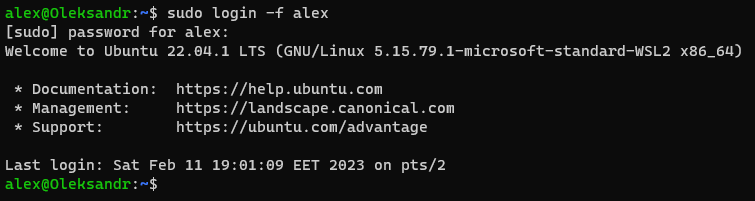
\includegraphics[width=0.7\linewidth]{Prt sc/Figure_1.png}  
        \end{minipage}
    \end{figure}

    \begin{center}
        \Large{Task \RomanNumeralCaps{2}}
    \end{center}
    Поміняйте ваш пароль. Ваш новий пароль повинен включати в себе як частину номер Вашої залікової книжки.
    \begin{figure}[h!]
        \begin{minipage}[h]{1\linewidth}
            \centering
            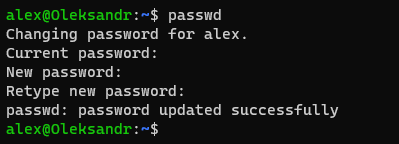
\includegraphics[width=0.7\linewidth]{Prt sc/Figure_2.png}  
        \end{minipage}
    \end{figure}

    \begin{center}
        \Large{Task \RomanNumeralCaps{3}}
    \end{center}
    Виведіть системну дату.
    \begin{figure}[h!]
        \begin{minipage}[h]{1\linewidth}
            \centering
            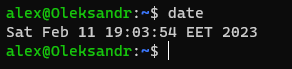
\includegraphics[width=0.6\linewidth]{Prt sc/Figure_3.png}  
        \end{minipage}
    \end{figure}

    \begin{center}
        \Large{Task \RomanNumeralCaps{4}}
    \end{center}
    Підрахуйте кількість рядків у файлі: \textbf{/etc/rsyslog.conf}
    \begin{figure}[h!]
        \begin{minipage}[h]{1\linewidth}
            \centering
            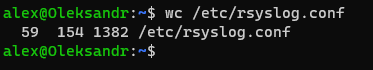
\includegraphics[width=0.7\linewidth]{Prt sc/Figure_4.png}  
        \end{minipage}
    \end{figure}

\newpage
    \begin{center}
        \Large{Task \RomanNumeralCaps{5}}
    \end{center}
    Виведіть на екран вміст відповідного файлу.
    \begin{figure}[h!]
        \begin{minipage}[h]{1\linewidth}
            \centering
            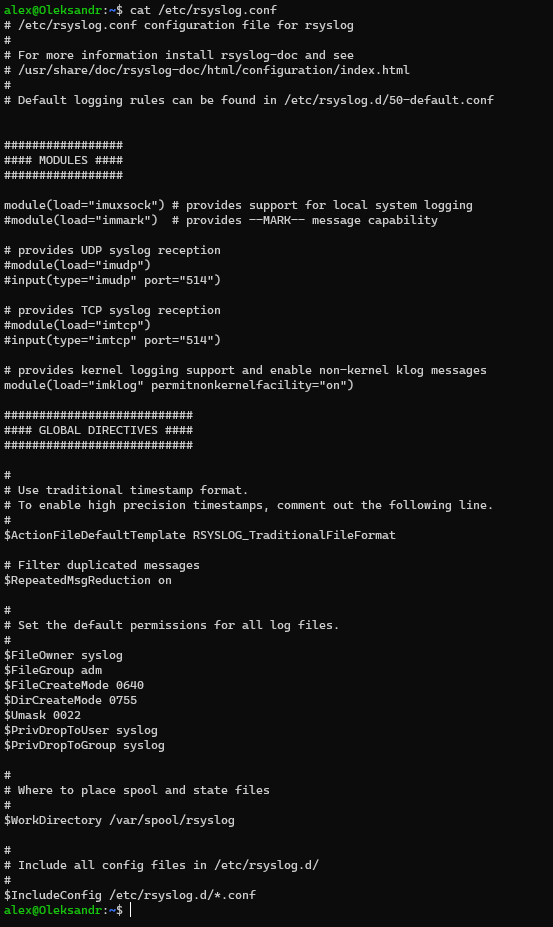
\includegraphics[width=0.7\linewidth]{Prt sc/Figure_5.png}  
        \end{minipage}
    \end{figure}

\newpage
    \begin{center}
        \Large{Task \RomanNumeralCaps{6}}
    \end{center}
    Виведіть календар на \textbf{2000} рік.
    \begin{figure}[h!]
        \begin{minipage}[h]{1\linewidth}
            \centering
            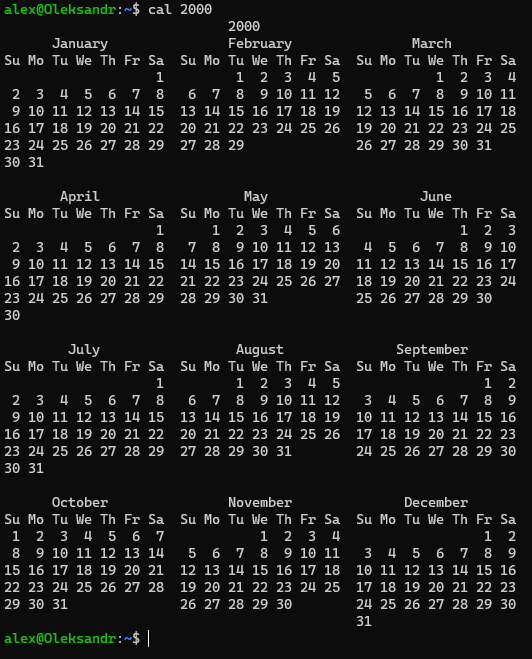
\includegraphics[width=0.6\linewidth]{Prt sc/Figure_6.png}  
        \end{minipage}
    \end{figure}
    
    \begin{center}
        \Large{Task \RomanNumeralCaps{7}}
    \end{center}
    Виведіть календар на 1752 рік. Чи не помічаєте що-небудь цікаве у вересні? Поясніть.
    \begin{figure}[h!]
        \begin{minipage}[h]{1\linewidth}
            \centering
            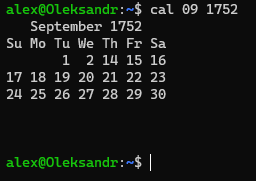
\includegraphics[width=0.4\linewidth]{Prt sc/Figure_7.png}  
        \end{minipage}
    \end{figure} \\
    Ми бачимо, що немає днів з 2 по 14 числа. Це тому, що саме тоді Велика Британія перейшла 
    з юліанського календаря на григоріанський календар.

\newpage
    \begin{center}
        \Large{Task \RomanNumeralCaps{8}}
    \end{center}
    Визначте, хто ще завантажений у систему.
    \begin{figure}[h!]
        \begin{minipage}[h]{1\linewidth}
            \centering
            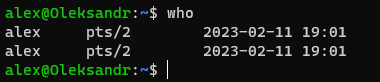
\includegraphics[width=0.5\linewidth]{Prt sc/Figure_8.png}  
        \end{minipage}
    \end{figure}
    
    \begin{center}
        \Large{Task \RomanNumeralCaps{9}}
    \end{center}
    Наберiть команду ping. Пояснiть результат.
    \begin{figure}[h!]
        \begin{minipage}[h]{1\linewidth}
            \centering
            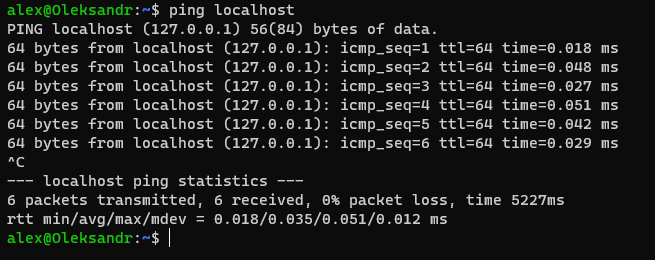
\includegraphics[width=0.8\linewidth]{Prt sc/Figure_9.png}  
        \end{minipage}
    \end{figure} \\
    У Linux команда ping є загальною утилітою, яка використовується для перевірки 
    наявності будь-якої мережі та чи доступний хост. За допомогою цієї команди ми 
    можемо перевірити, чи працює сервер і чи він виконується. Крім того, це допомагає визначити
    затримку <<latency>>.
    Для перевірки інтерфейсу локальної мережі ми можемо використовувати будь-який з наступних способів:
    \begin{enumerate}
        \item ping 0
        \item ping localhost
        \item ping 127.0.0.1
    \end{enumerate}

    \begin{center}
        \Large{Task \RomanNumeralCaps{10}}
    \end{center}
    Скопіюйте файли: \textbf{/bin/more}, \textbf{/bin/gzip} у ваш домашній каталог різними способами.
    \begin{figure}[h!]
        \begin{minipage}[h]{1\linewidth}
            \centering
            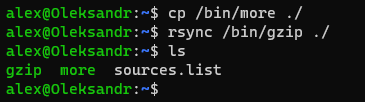
\includegraphics[width=0.6\linewidth]{Prt sc/Figure_10.png}  
        \end{minipage}
    \end{figure}

\newpage
    \begin{center}
        \Large{Task \RomanNumeralCaps{11}}
    \end{center}
    Створiть каталог \textbf{lab\_1}.
    \begin{figure}[h!]
        \begin{minipage}[h]{1\linewidth}
            \centering
            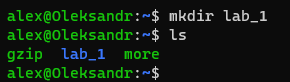
\includegraphics[width=0.6\linewidth]{Prt sc/Figure_11.png}  
        \end{minipage}
    \end{figure}

    \begin{center}
        \Large{Task \RomanNumeralCaps{12}}
    \end{center}
    \textbf{Скопiюйте} в нього з вашого домашнього каталогу копiю файлу 1, яку ви отримали в
    п.10, пiд iм’ям \textbf{my\_more}. \textbf{Перемiстiть} в цей каталог з вашого домашнього каталогу
    копiю файлу 2, яку ви отримали в п.10, перейменувавши його при цьому в \textbf{my\_gzip}.
    \begin{figure}[h!]
        \begin{minipage}[h]{1\linewidth}
            \centering
            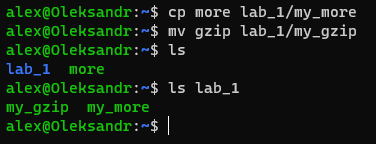
\includegraphics[width=0.6\linewidth]{Prt sc/Figure_12.png}  
        \end{minipage}
    \end{figure}

    \begin{center}
        \Large{Task \RomanNumeralCaps{13}}
    \end{center}
    Перейдіть у свій домашній каталог і переконайтеся в тому, що все зроблено правильно.
    \begin{figure}[h!]
        \begin{minipage}[h]{1\linewidth}
            \centering
            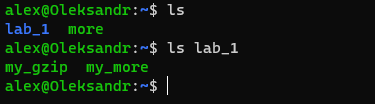
\includegraphics[width=0.6\linewidth]{Prt sc/Figure_13.png}  
        \end{minipage}
    \end{figure}

    \begin{center}
        \Large{Task \RomanNumeralCaps{14}}
    \end{center}
    Створіть каталог \textbf{lab\_1\_5} і перейдіть в нього.
    \begin{figure}[h!]
        \begin{minipage}[h]{1\linewidth}
            \centering
            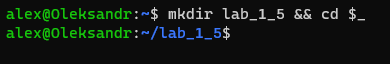
\includegraphics[width=0.6\linewidth]{Prt sc/Figure_14.png}  
        \end{minipage}
    \end{figure}

\newpage
    \begin{center}
        \Large{Task \RomanNumeralCaps{15}}
    \end{center}
    Скопіюйте в каталог \textbf{lab\_1\_5} файл з п.4 під ім'ям \textbf{nrsyslog.conf}.
    \begin{figure}[h!]
        \begin{minipage}[h]{1\linewidth}
            \centering
            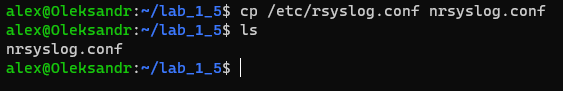
\includegraphics[width=0.6\linewidth]{Prt sc/Figure_15.png}  
        \end{minipage}
    \end{figure}

    \begin{center}
        \Large{Task \RomanNumeralCaps{16}}
    \end{center}
    За допомогою команд cat і less перегляньте його вміст.
    \begin{figure}[h!]
        \begin{minipage}[h]{1\linewidth}
            \centering
            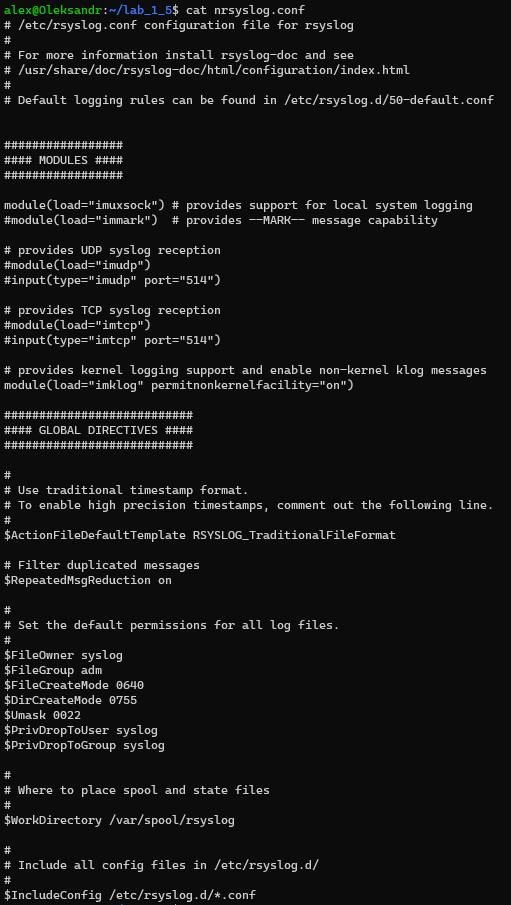
\includegraphics[width=0.6\linewidth]{Prt sc/Figure_16.png}  
        \end{minipage}
        \caption{Результат виконання команди cat.}
    \end{figure}

\newpage
    \begin{figure}[h!]
        \begin{minipage}[h]{1\linewidth}
            \centering
            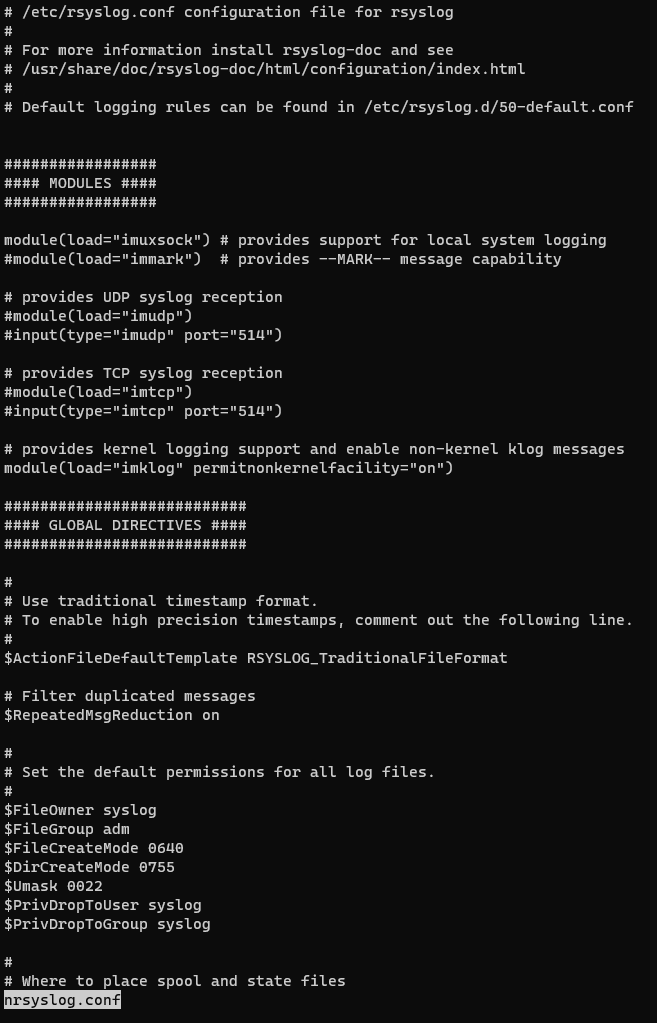
\includegraphics[width=0.6\linewidth]{Prt sc/Figure_17.png}  
        \end{minipage}
        \caption{Результат виконання команди less.}
    \end{figure}
    Різниця між командами полягає в тому, що less — програма для читання файлів, 
    а cat — програма для обробки рядків.

    \begin{center}
        \Large{Task \RomanNumeralCaps{18}}
    \end{center}
    Перейдіть у свій домашній каталог.
    \begin{figure}[h!]
        \begin{minipage}[h]{1\linewidth}
            \centering
            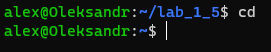
\includegraphics[width=0.6\linewidth]{Prt sc/Figure_18.png}  
        \end{minipage}
    \end{figure}

\newpage
    \begin{center}
        \Large{Task \RomanNumeralCaps{19}}
    \end{center}
    Видаліть каталог \textbf{lab\_1\_5}.
    \begin{figure}[h!]
        \begin{minipage}[h]{1\linewidth}
            \centering
            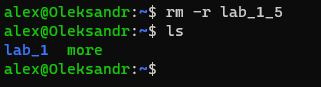
\includegraphics[width=0.6\linewidth]{Prt sc/Figure_19.png}  
        \end{minipage}
    \end{figure}

    \begin{center}
        \Large{Висновки}
    \end{center}

    Підсумовуючи виконану роботу зрозуміло, що використання базових команд в 
    повсякденному житті для звичайного користувача не є практичним. В більшості випадків 
    набагато простіше перемістити/скопіювати/переглянути файл через графічний інтерфейс. 
    Відповідно по місцю його перейменувати.

    Проте не всі дистибутиви Linux мають з коробки графічний інтерфейс. 
    З дебільшого ОС Linux використовується на мейнфреймах, суперкомп'ютерах,
    для вебсерверів тощо. І в цьому випадку використовується здебільшого термінал. 
    Тому базові команди є незамінними.
    \begin{center}
        Розгляд команд
    \end{center}

    Команда 'man' краще підходить для швидкого перегляду атрибутів команди та її опису. 
    В свою чергу 'info' дає повний опис відповідної команди.
    
    'passwd' цілком зручна команда для зміни паролю без використання графічного інтерфейсу
    з утриманням відповідних умов складності нового паролю. Хоча при створення нового 
    користовуча можна задавати пароль будь-якої складності.
    
    Команди 'cal', 'date', 'ls', 'cd', 'cp', 'mv', 'mkdir', 'rm', 'rmdir' найчастіше
    зустічаються та використовуються користовучами, їх функціонал максимально оптимізований,
    простий та зручний.
    
    'cat', 'less' - команди обробки змісту файлів. Перша більше підходить для ознайомлення з 
    невеликими за обсягом файлами, адже незручно переглядати великі файли в терміналі без
    змоги переміщати курсор по рядкам. В свою чергу 'less' це програма для читання файлів,
    тому максимально оптимізована для перегляду великих файлів. Для отримання поверхневої
    інформації щодо файлу можна використати 'wc'.
    
    Загалом всі команди складають початковий набір будь-якого користувача ОС Linux і не тільки. 
    Тому їх функціонал та простота повинна бути доступна для кожного нового юзера, що відповідає дійсності.
\end{document}